\documentclass[tikz]{standalone}
\usepackage{tikz}
\pgfmathsetmacro{\n}{25}

\begin{document}
  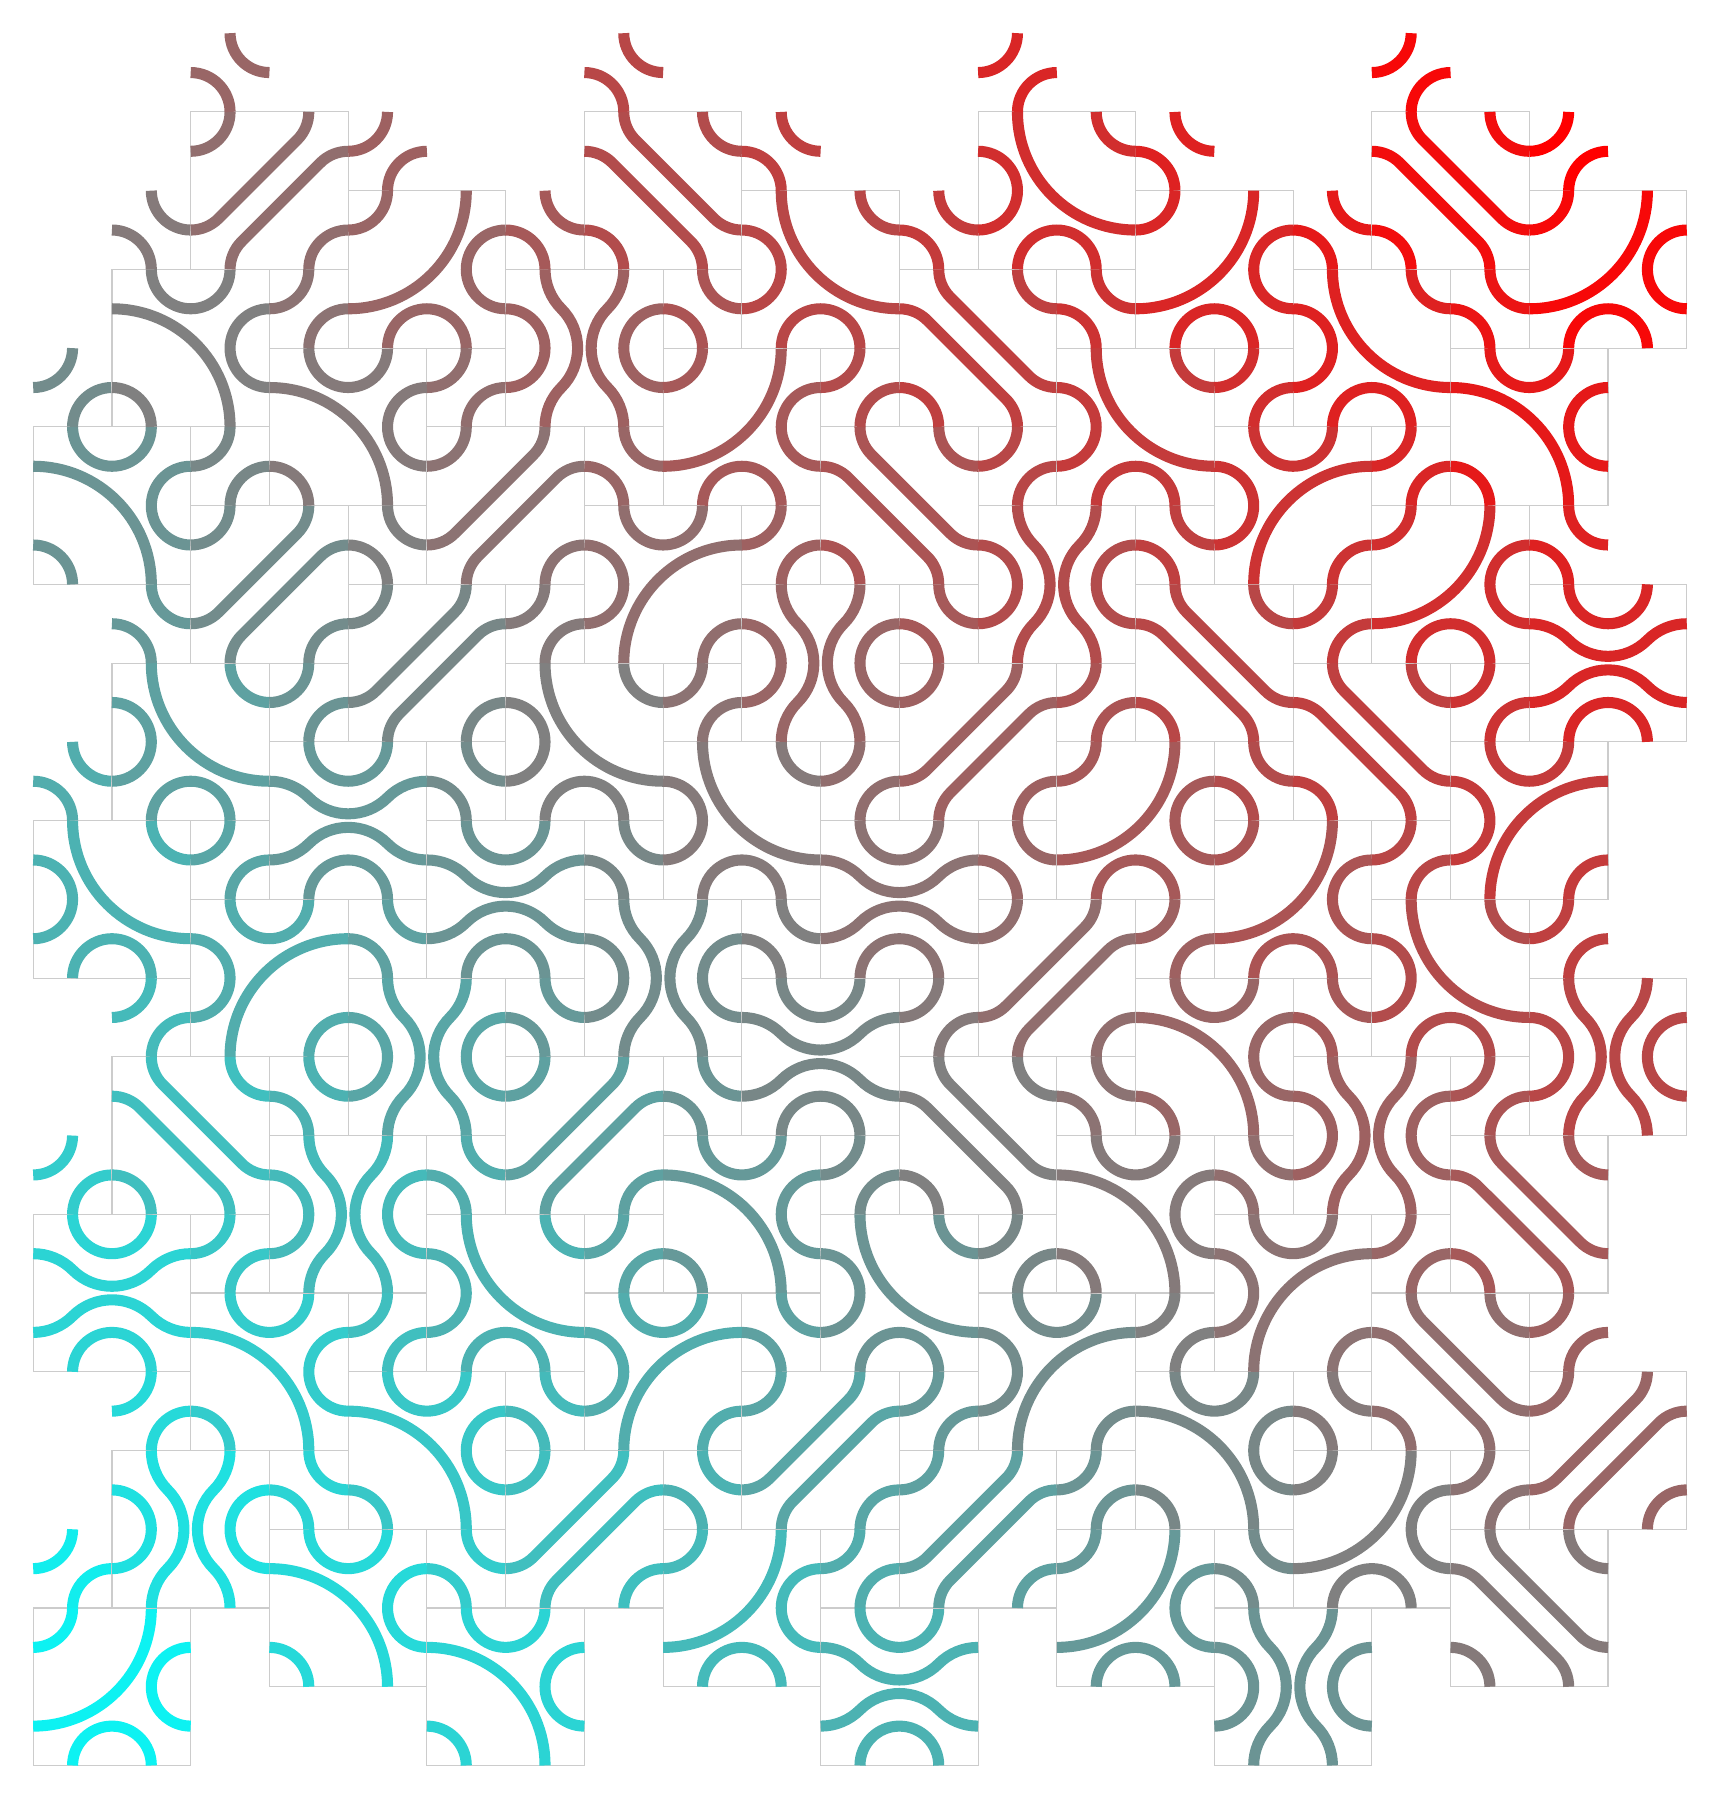
\begin{tikzpicture}
    \foreach \x [
      evaluate={\ymin using {mod(2*\x,5)}}
    ] in {0,...,19} {
      \foreach \i [
        evaluate={\y using int(5*\i + \ymin)},
        evaluate={\s using random(0,7)},
        evaluate={\t using random(0,1)},
        evaluate={\colorA using int(2.5*(\x+\y+2))},
        evaluate={\colorB using int(2.5*(\x+\y+3))},
      ] in {0,...,3} {
        \draw[black!20] (\x,\y) rectangle (\x+2,\y+2);
        \ifnum \s<2 {
          % Type I
          \draw[line width=4, red!\colorA!cyan, rotate around={90*\s:(\x+1,\y+1)}]
            (\x+1/2,\y) arc (180:135:1/2) -- ({\x+2-sqrt(2)/4},{\y+2/2+sqrt(2)/4}) arc (135:90:1/2)
            (\x+3/2,\y) arc (180:90:1/2)
            (\x,\y+1/2) arc (270:315:1/2) -- ({\x+2/2+sqrt(2)/4},{\y+2-sqrt(2)/4}) arc (315:360:1/2)
            (\x,\y+3/2) arc (270:360:1/2)
          ;
        } \else {
          \ifnum \s<4 {
            % Type II
            \draw[line width=4, red!\colorA!cyan, rotate around={90*\s:(\x+1,\y+1)}]
              (\x+1/2,\y) arc (180:0:1/2)
              (\x+1/2,\y+2) arc (180:360:1/2)
              (\x,\y+1/2) arc (270:315:0.707) arc (135:45:0.707) arc (225:270:0.707)
              (\x,\y+3/2) arc (90:45:0.707) arc (225:315:0.707) arc (135:90:0.707)
            ;
          } \else {
            % Type III
            \draw[line width=4, red!\colorA!cyan, rotate around={90*\s:(\x+1,\y+1)}]
              (\x+1/2,\y) arc (180:90:3/2)
              (\x+3/2,\y) arc (180:90:1/2)
              (\x,\y+1/2) arc (-90:90:1/2)
              (\x+1/2,\y+2) arc (180:360:1/2)
            ;
          } \fi
        } \fi
        \draw[line width=4, red!\colorB!cyan, rotate around={90*\t:(\x+1/2,\y+5/2)}]
          (\x+1/2,\y+2) arc (180:90:1/2)
          (\x,\y+5/2) arc (270:360:1/2)
        ;
        % \node at (\x+1,\y+1) {\x, \y, \colorA};
        % \node at (\x+1/2,\y+5/2) {\x, \y, \colorB};
      }
    }
  \end{tikzpicture}
\end{document}
